\section{Bericht}

\subsection{Einleitung}
Ziel der Übung ist es den Winkel $\alpha$ als Funktion, abhängig vom Winkel $\beta$ zu bestimmen und einen Graphen der Funktion $\alpha = f(\beta)$ darzustellen. Der Graph soll im Bereich $\beta = -300$ Grad bis $\beta = +300$ Grad gezeichnet werden. \\
Gegeben ist uns eine Versuchsbeschreibung mit detaillierten Grafiken zur Geometrie.

\subsection{Durchführung}
\begin{center}
	\begin{minipage}{\linewidth}
	\centering
	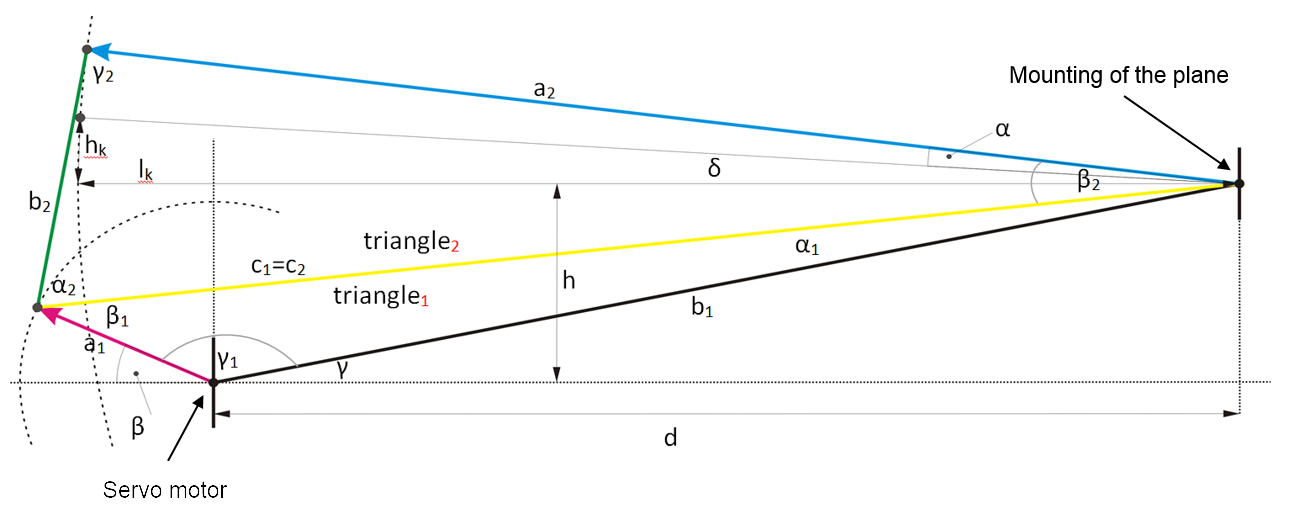
\includegraphics[scale=0.3]{images/figure1.png}
	\captionof{figure}{Model of inclined plane}
	\end{minipage}
\end{center}
Um die gestellt Aufgabe zu schaffen, haben wir mit Hilfe der gegebenen Formeln und Abbildungen zuerst die Funktion aufgestellt und mit dieser ein Scilab-Skript geschrieben, welches den Graphen abbildet.\\
Zuerst haben wir die Formel $\beta + \gamma_1 + \gamma = \pi$ nach $\gamma_1$ umgestellt. Da der Wert für $\gamma = arctan(\frac{h}{d})$ konstant und $\beta$ der Winkel des Motorarms ist ($\beta$ ist zwischen $-300$ Grad und $+300$ Grad), können wir den Wert für $\gamma_1$ und ein bestimmtes $\beta$ direkt errechnen. Wir erhalten also ein Dreieck, in dem uns die Länge der beiden Katheten ($a_1$, $b_1$) und der Wert des eingeschlossenen Winkels ($\gamma_1$) bekannt sind. \\
Nach dem Kosinussatz können wir nun die Hypotenuse berechnen:\\ ${c_1}^2 = {a_1}^2 + {b_1}^2 -2a_1b_1cos(\gamma_1) \Rightarrow c_1 = \sqrt{{a_1}^2 + {b_1}^2 -2a_1b_1cos(\gamma_1)}$ \\
Nach dem gleichen Prinzip lässt sich nun auch der Winkel $\beta_2$ berechnen:\\
${b_2}^2 = {a_2}^2 + {c_1}^2 - 2a_2 c_1 cos(\beta_2) \Rightarrow \beta_2 = arccos(\frac{{a_2}^2 + {c_1}^2 - {b_2}^2}{2a_2 c_1})$\\
Um $\alpha$ zu berechnen benötigen wir den noch fehlenden Winkel $\alpha_1$. Dieser wird nach der Formel \\
${a_1}^2 = {c_1}^2 + {b_1}^2 - 2c_1 b_1 cos(\alpha_1) \Rightarrow \alpha_1 = arccos(\frac{{c_1}^2+{b_1}^2-{a_1}^2}{2c_1 b_1})$ \\
berechnet.\\
Schlussendlich kann die Formel $\alpha + \delta + \gamma = \alpha_1 + \beta_1$ nach $\alpha = \alpha_1 +\beta_1 - \delta - \gamma$ umgestellt werden und man erhält damit den gesuchten Winkel $\alpha$ in Abhängigkeit von dem Winkel $\beta$.

\subsection{Besonderheiten}
Im Versuch sind vier verschiedene Fälle zu betrachten, da nicht alle gegeben Formeln immer zutreffen.\\ Ist zum Beispiel der Winkel $\beta$ im Bereich $-\gamma > \beta > -\gamma -\pi$ muss die Formel $\beta + \gamma_1 + \gamma = \pi$ berichtigt werden. In diesem Bereich gilt: $\gamma_1 - \beta - \gamma = \pi$. Außerdem muss die Formel für $\alpha_1$ angepasst werden: $\alpha_1 = -arccos(\frac{{c_1}^2+{b_1}^2-{a_1}^2}{2c_1 b_1})$ \\
Überschreitet $\beta$ die schwarze Linie $b_1$ ($\beta < -\gamma - \pi$), gelten wieder die Ausgangsgleichungen (bis $-300$ Grad). \\
Analog müssen auch zwei Fälle in die positive Drehrichtung betrachtet werden ($-\gamma + \pi > \beta > -\gamma$ und $\beta > -\gamma + \pi$ bis $+300$ Grad).

\subsection{Fazit}
Da der für uns relevante Bereich für $\alpha$ zwischen $-5$ Grad und $+5$ Grad liegt, lässt sich die Kuve gut durch eine lineare Funktion mit $\alpha = \frac{a_1}{a_2}\beta$ approximieren. Lineare Funktionen lassen sich leichter implementieren und dadurch vereinfacht sich der Versuch erheblich.

 
%Diese Rechenschritte haben wir dann in einen Scilab Skript verwendet um den Graphen zu zeichnen. Mit Hilfe einer If-Abfrage konnten wir das Skript leicht abändern um eine Vergrößerung des Bereichs von Beta von ~40° auf ~300° zu vergrößern. Dies war nötig da man verschiedene Fälle betrachten muss wenn der Winkel Beta kleiner als -Gamma wird.